% gamla grejer - antagligen inte kört


\sectionslide{Dag 2 -- material!}


\frame{
\frametitle{Så funkar ett vridspoleinstrument -- Simpson}
    {\Huge Ett mätinstrument drar ström}
}


\frame{
\frametitle{Så funkar ett vridspoleinstrument -- principen}
    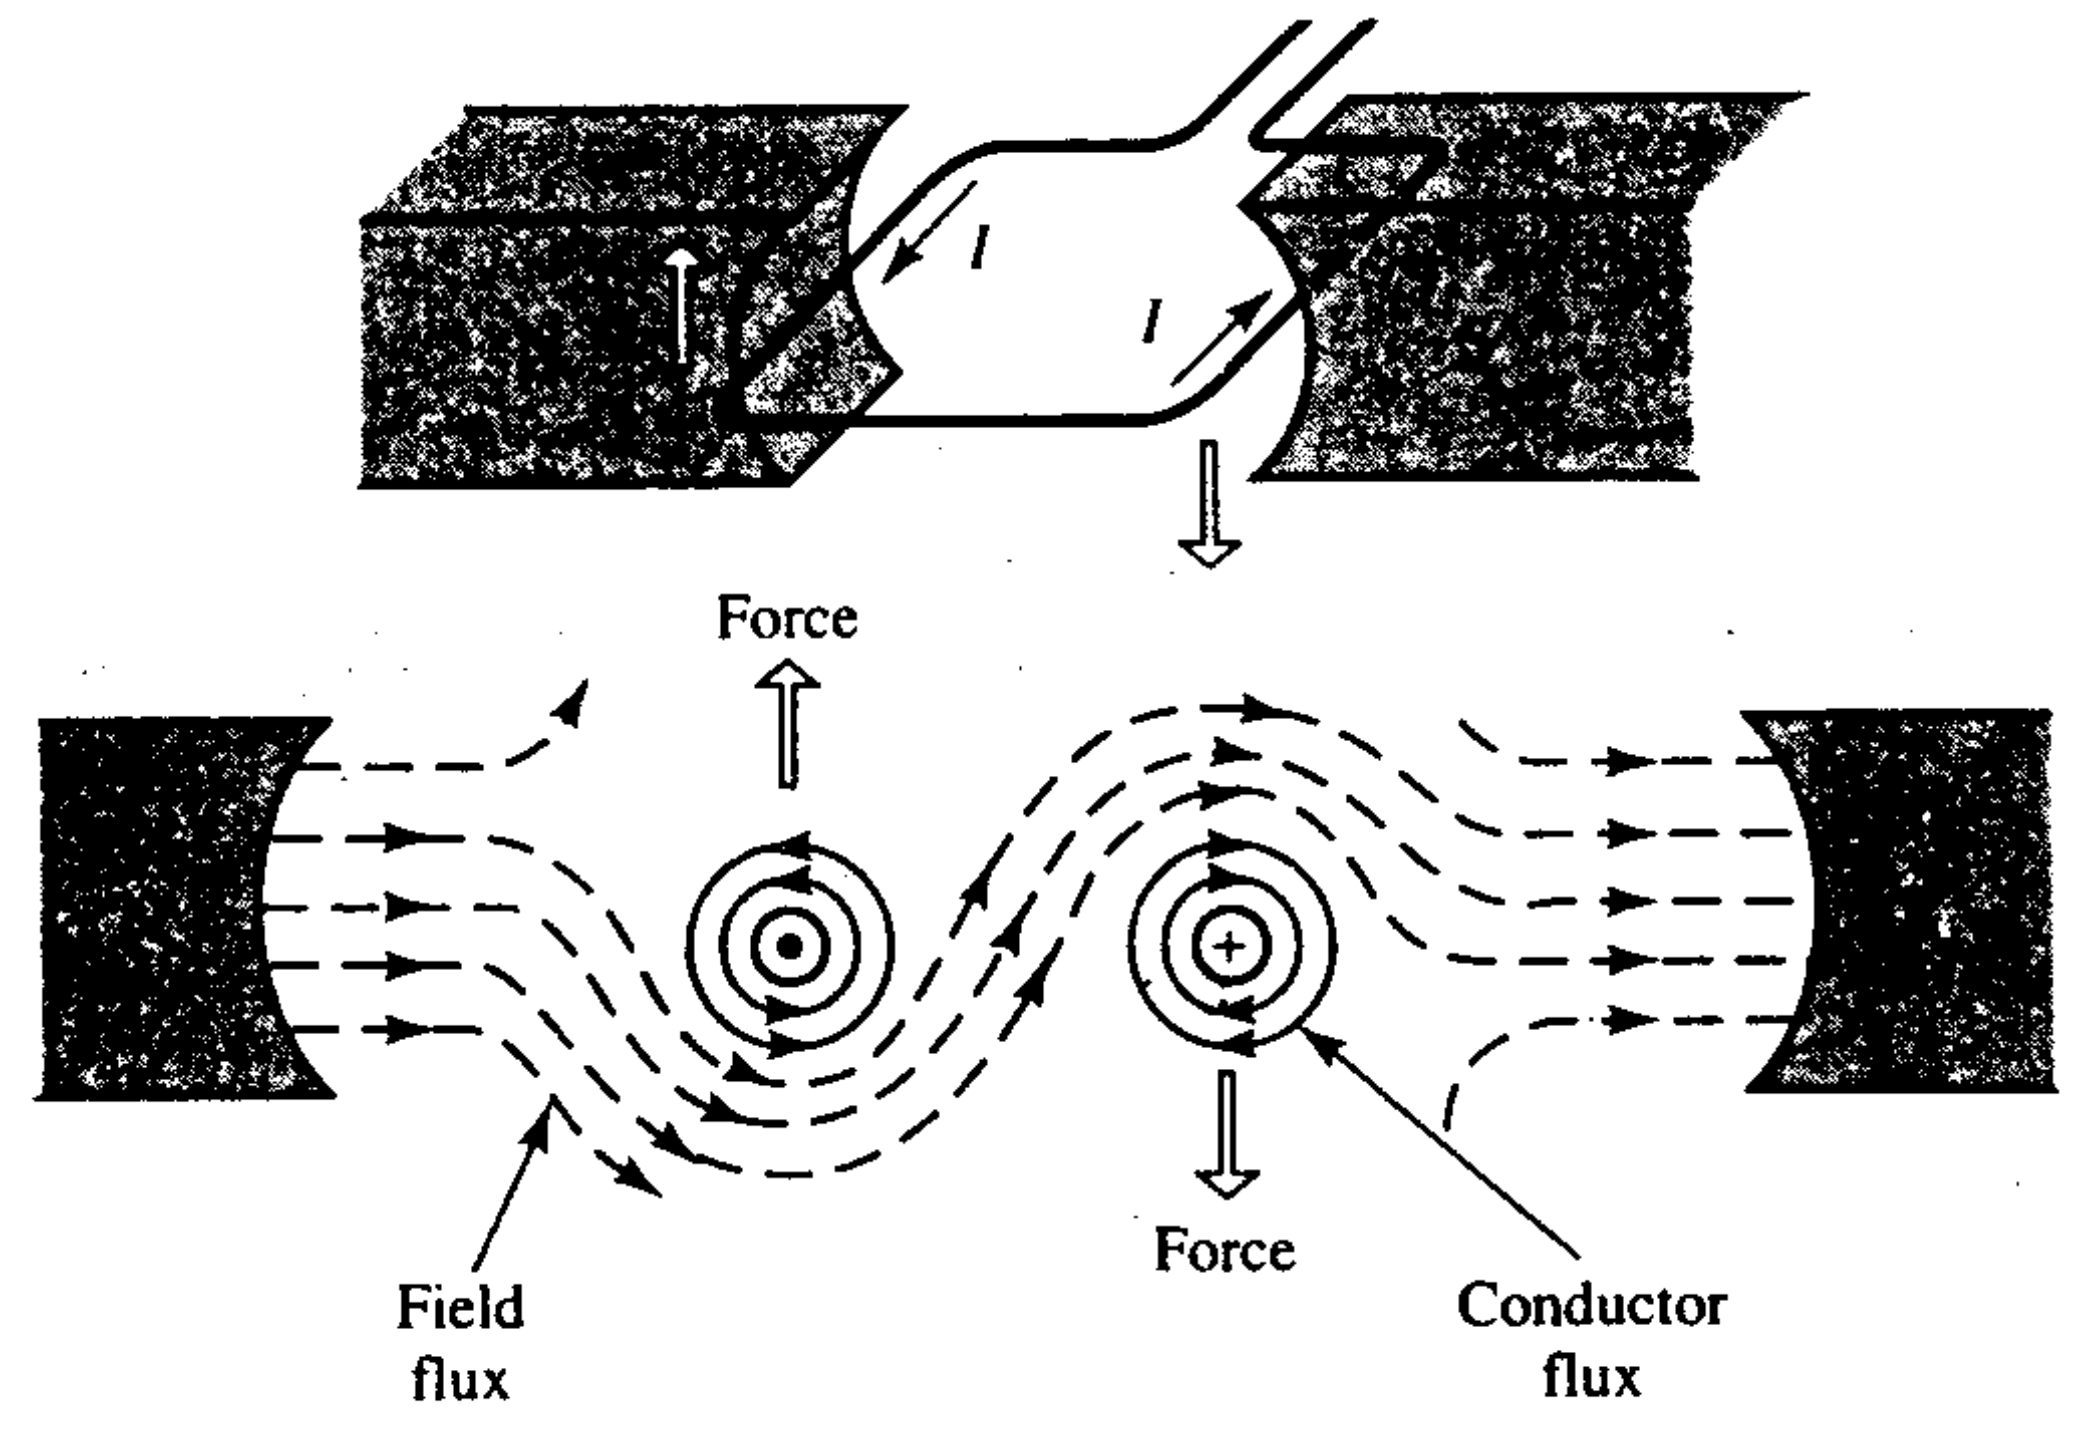
\includegraphics[width=\textwidth]{figures/stromslinga_i_magnetfalt.png}
}

\frame{
\frametitle{Så funkar ett vridspoleinstrument -- ingnejörskonsten}
    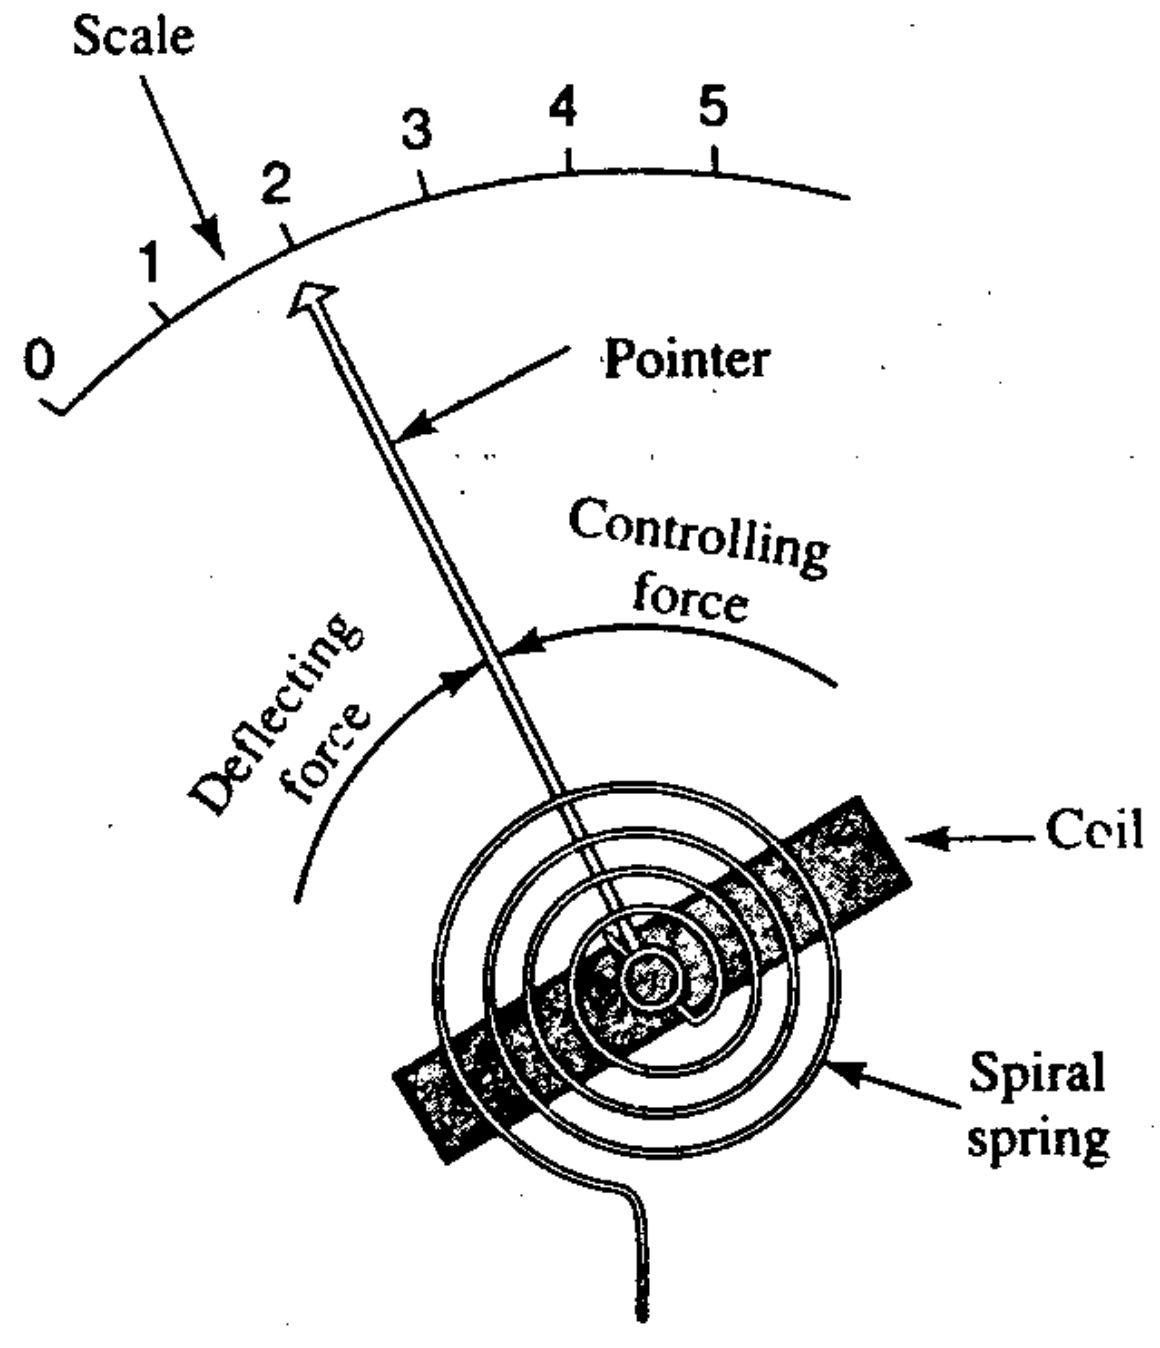
\includegraphics[width=0.45\textwidth]{figures/pmmc.png}
    \onslide<2->{
    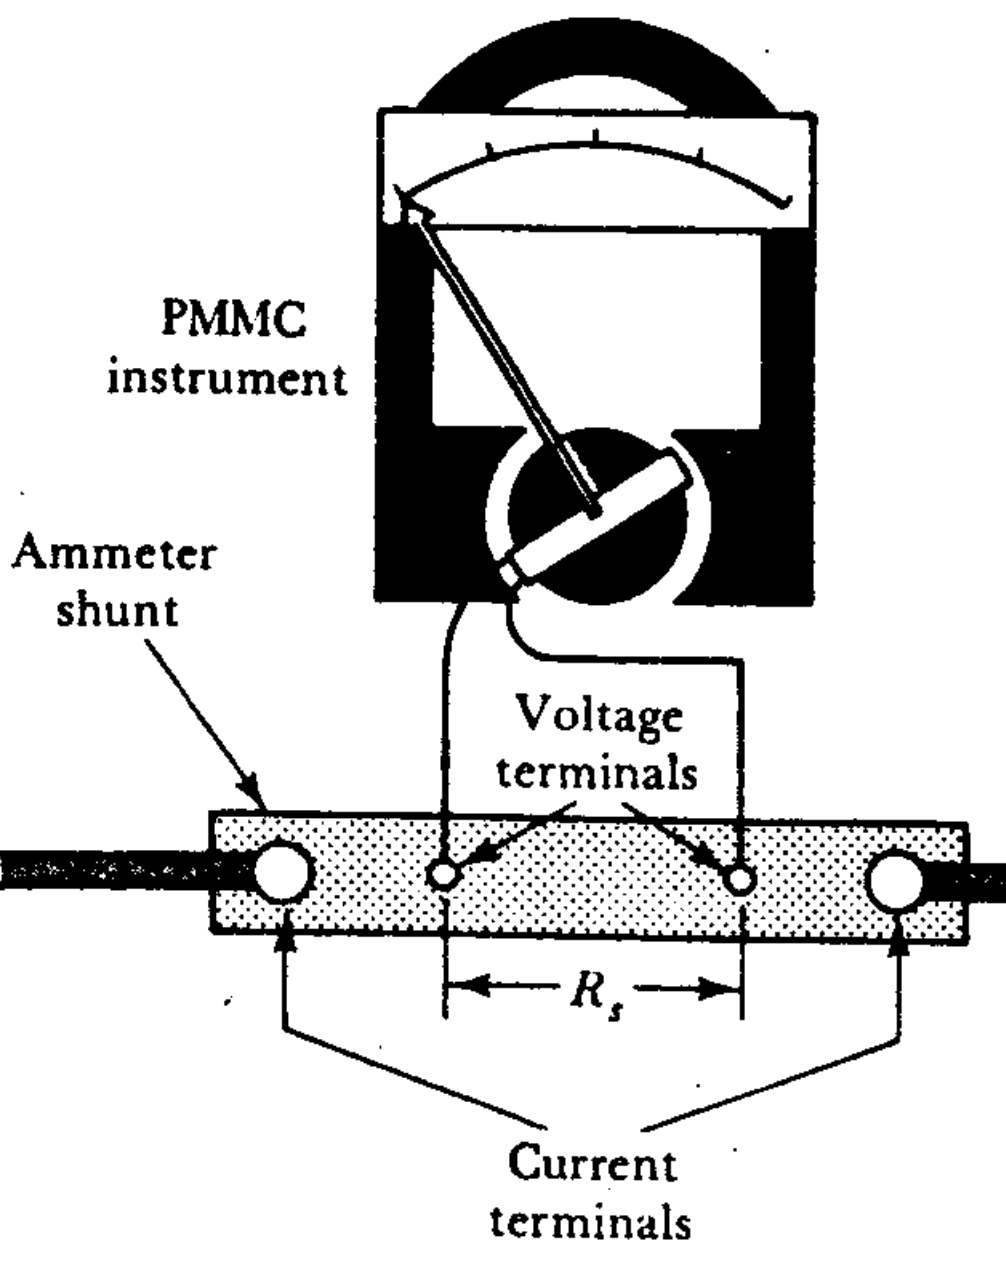
\includegraphics[width=0.45\textwidth]{figures/pmmc_instrument.png}
    }
}

\frame{
\frametitle{Så funkar ett vridspoleinstrument -- kretsen}
    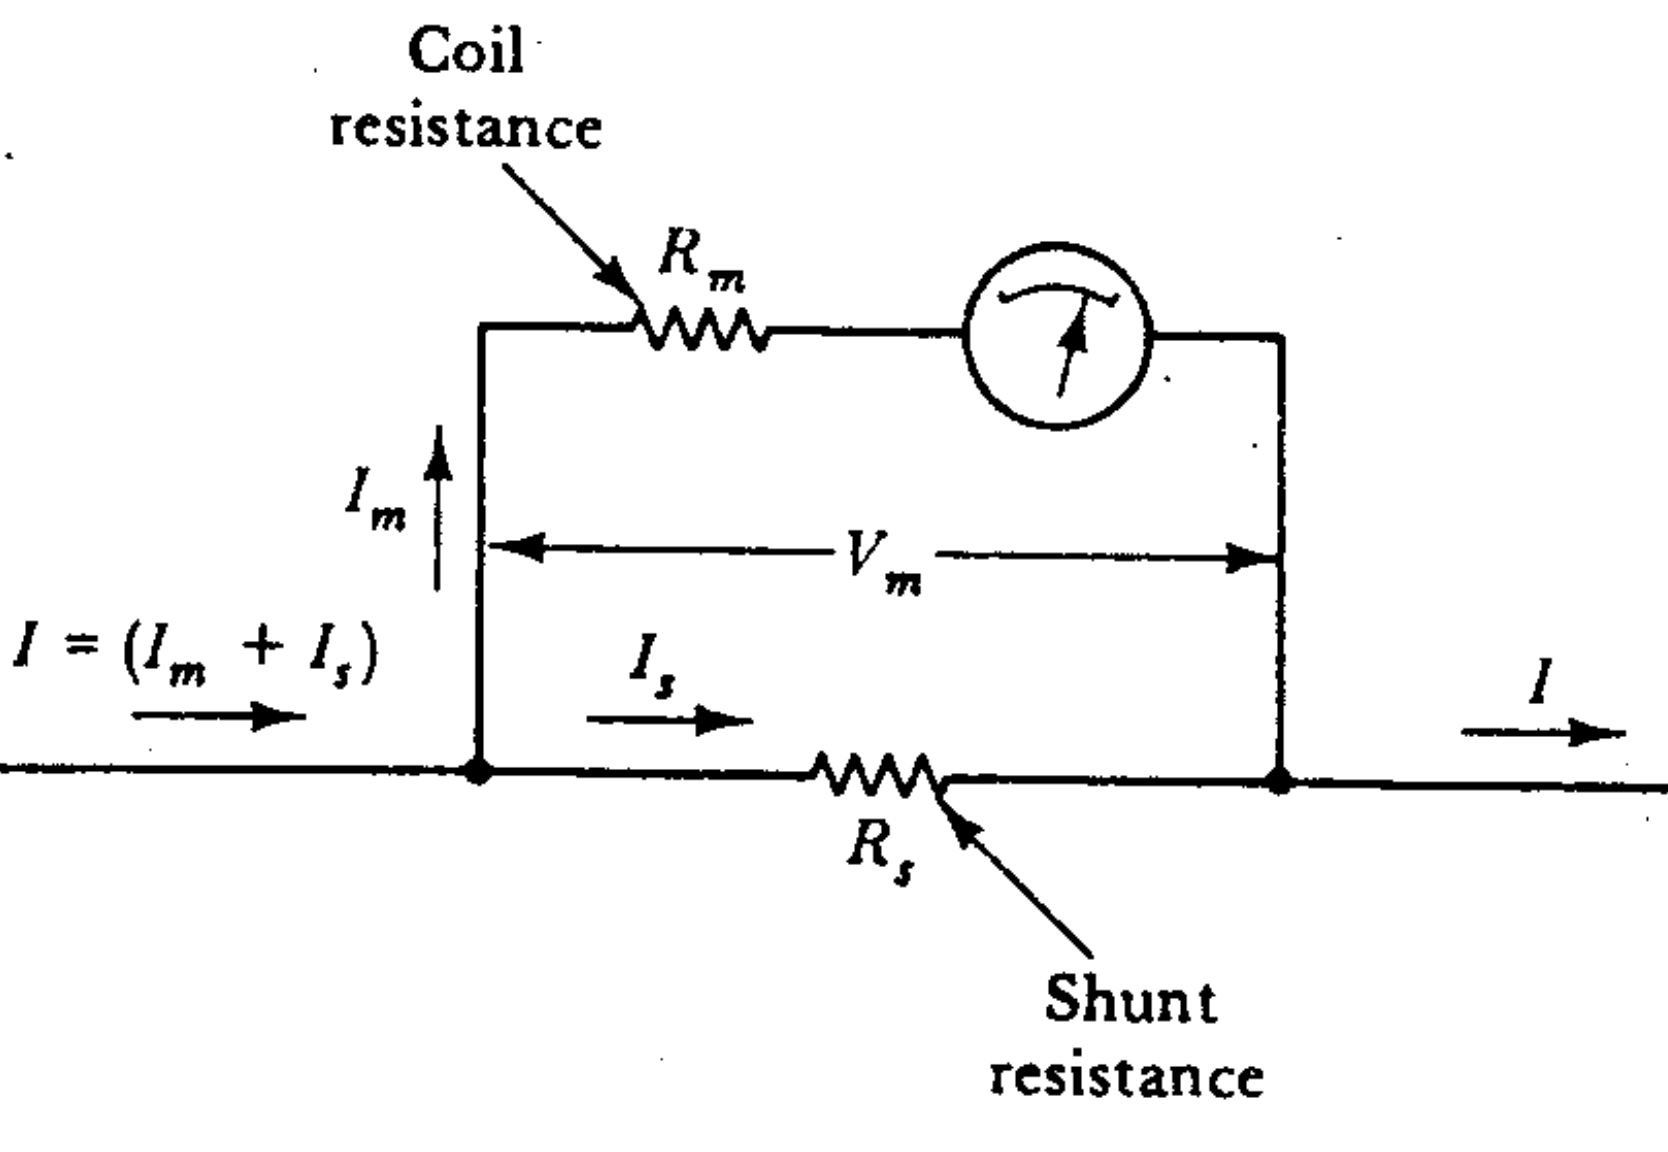
\includegraphics[width=\textwidth]{figures/pmmc_circuit.png}
}


\frame{
\frametitle{Så funkar ett vridspoleinstrument -- flera mätområden}
    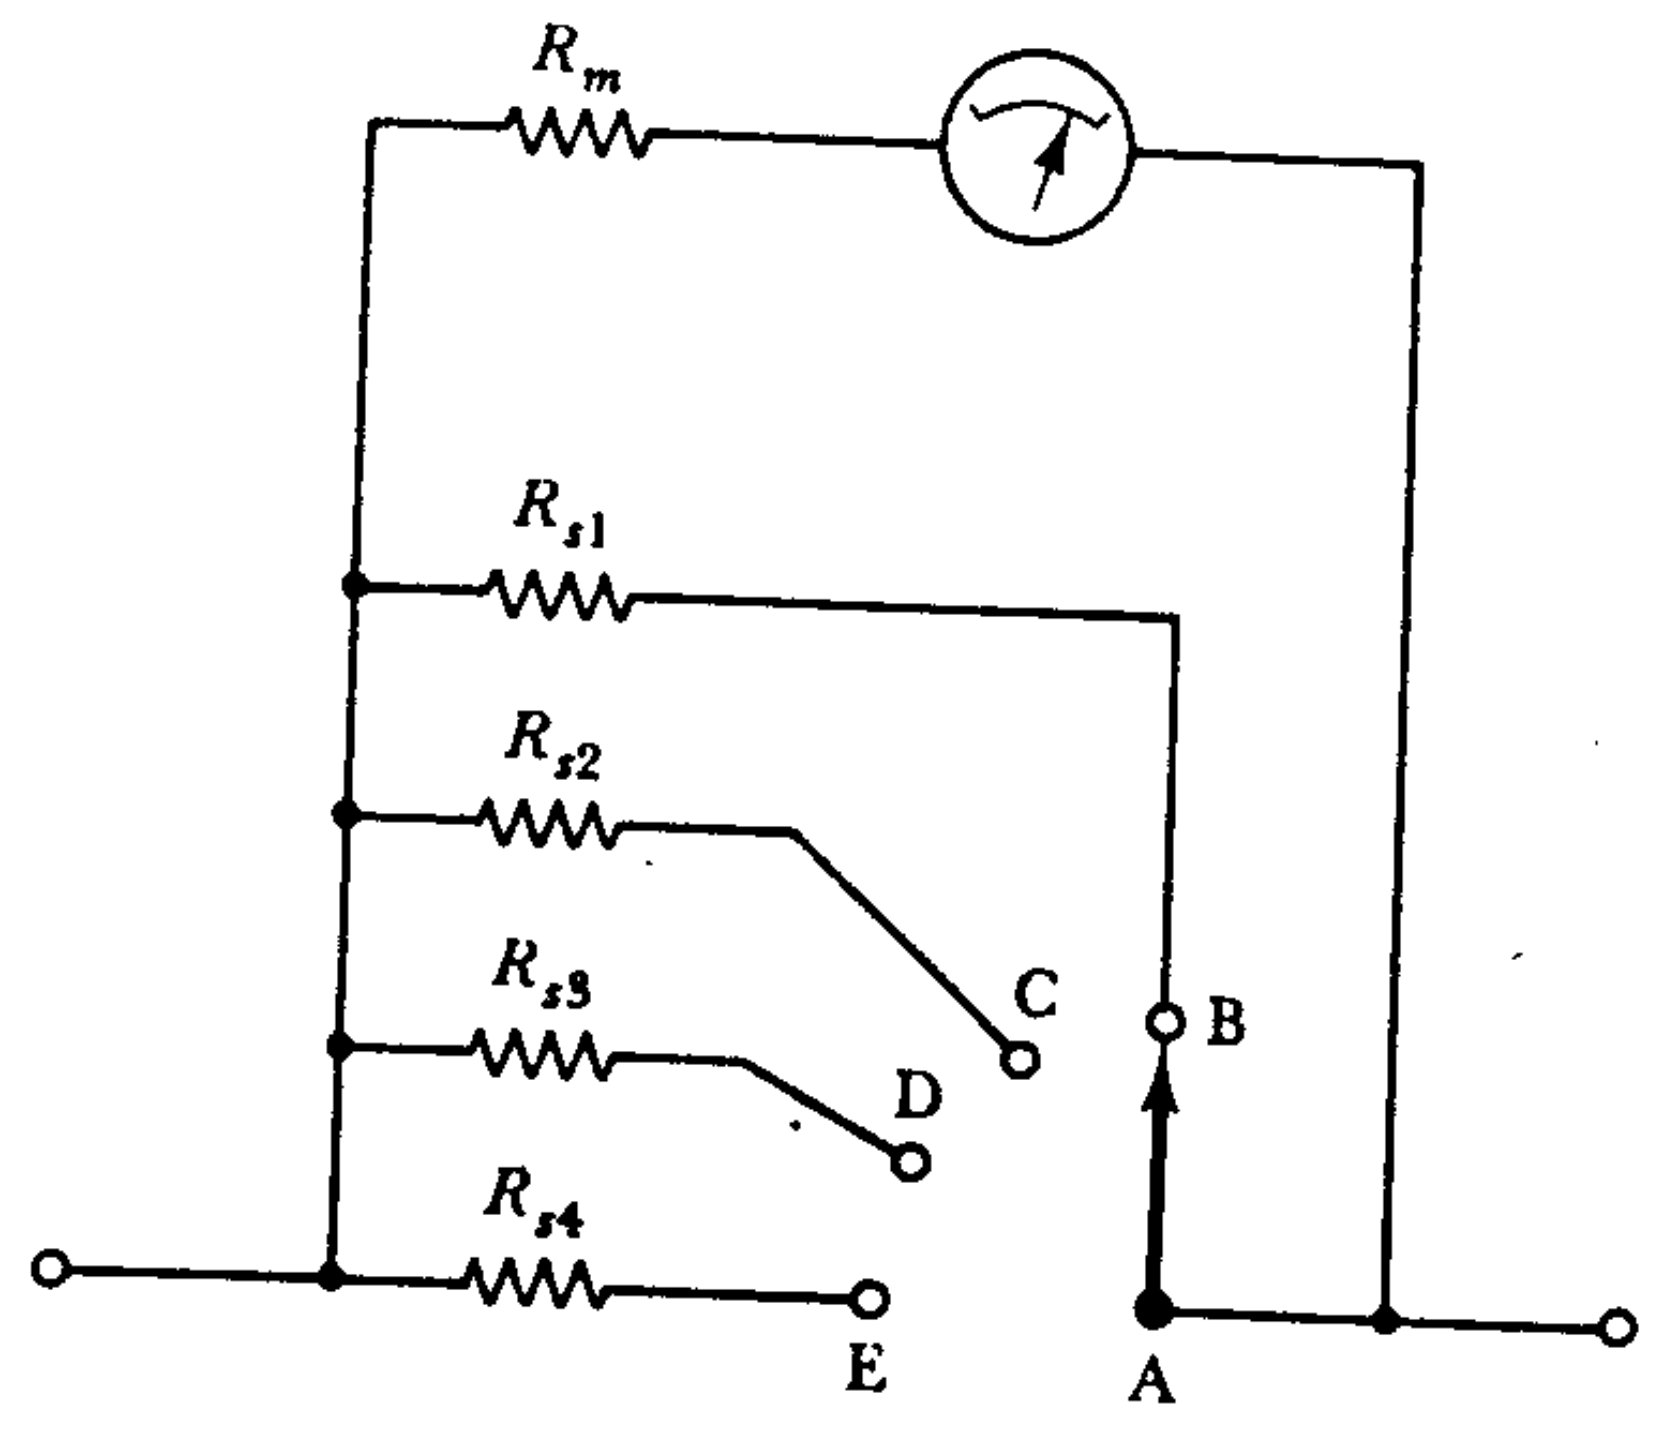
\includegraphics[width=0.8\textwidth, angle=2.5]{figures/pmmc_multirange.png}
}


\frame{
\frametitle{Bygg ett vridspoleinsrument}
}
